\section{PICK kết hợp văn bản ảnh và đồ thị}
PICK gồm ba phần: encoder, mô-đun đồ thị và decoder \parencite{yu2020}. Encoder kết hợp đặc trưng ký tự với đặc trưng ảnh của từng vùng chữ. Mỗi vùng trở thành một nút trong đồ thị; mô hình học mức liên hệ giữa các nút để bổ sung ngữ cảnh trước khi dự đoán nhãn.

\begin{figure}[htbp]
\centering
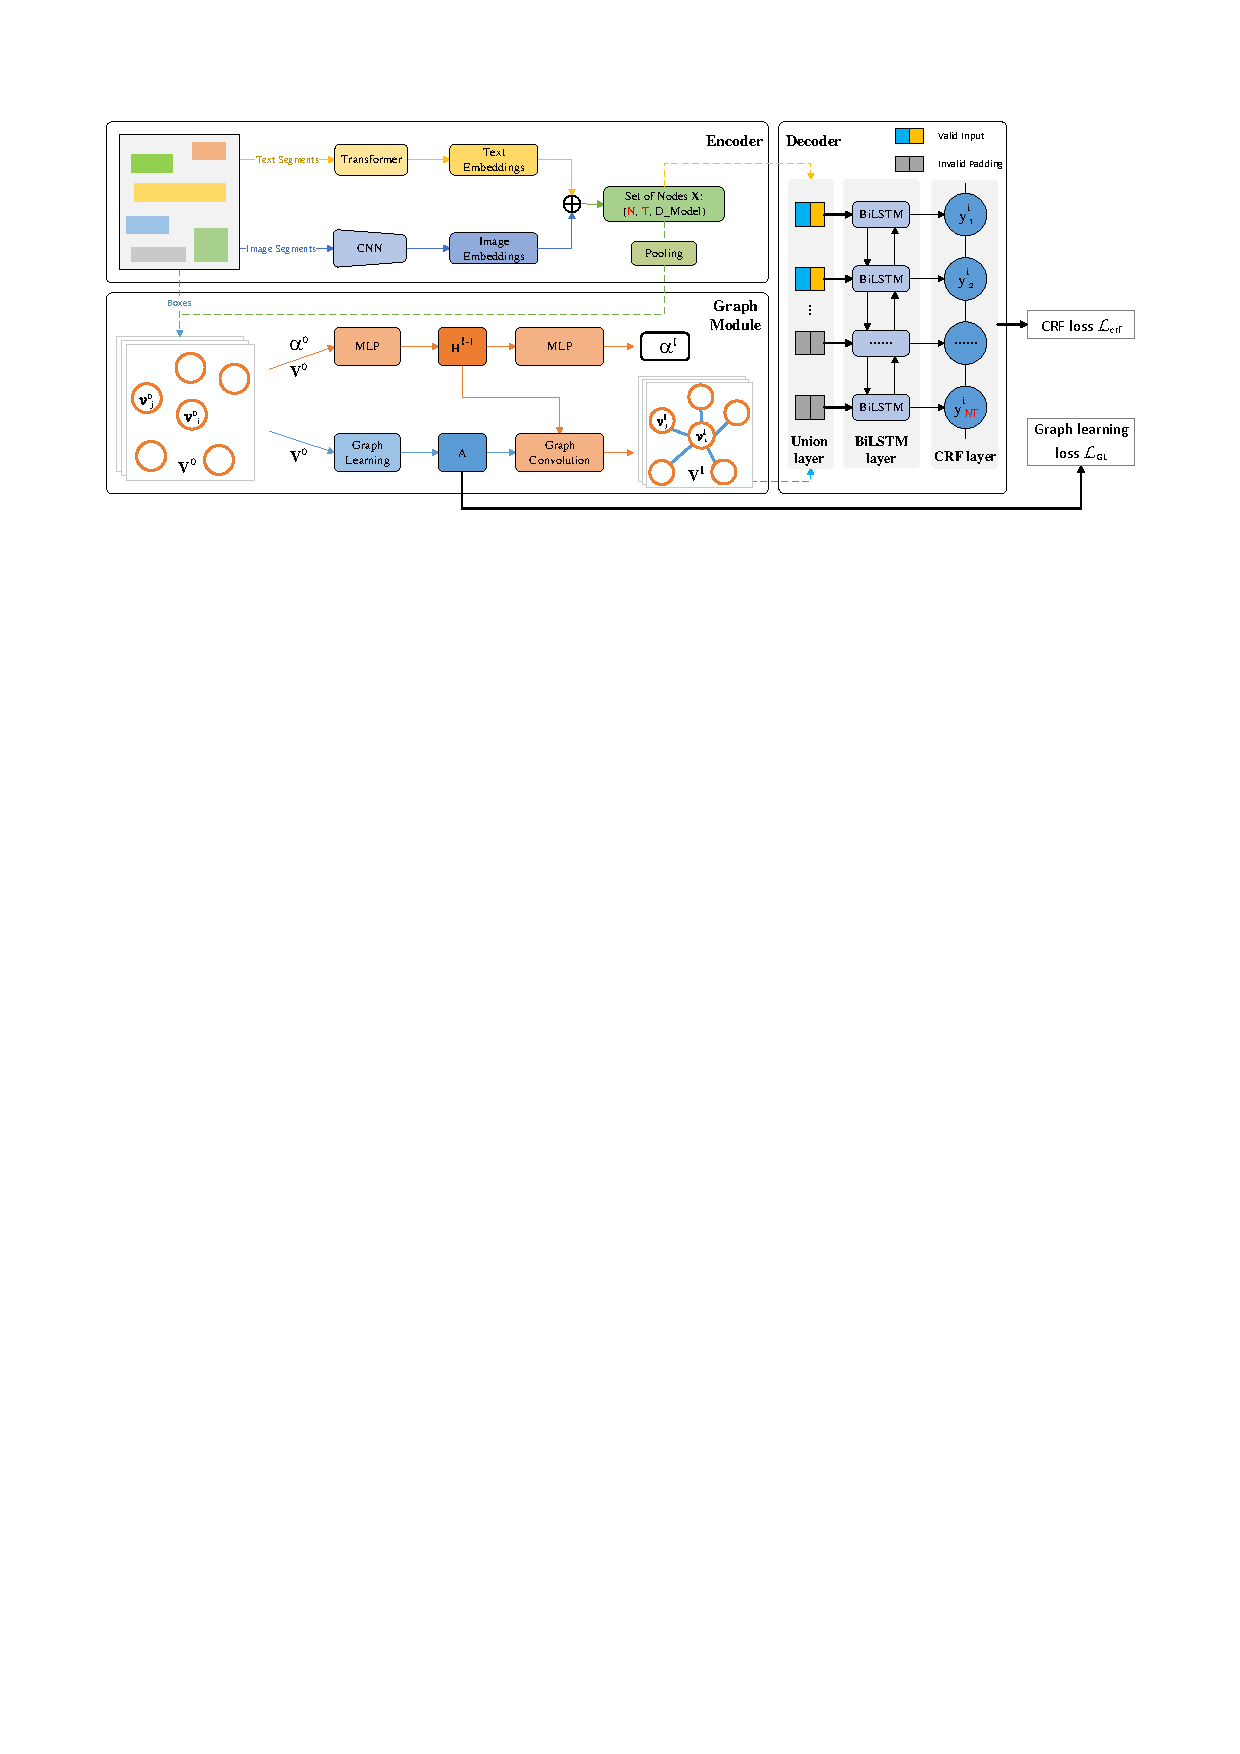
\includegraphics[width=\textwidth]{picture/pick-paper-figure-3.pdf}
\caption{Các thành phần chính của mô hình PICK}
\label{fig:pick-original}
\par\centering (Nguồn: \parencite{yu2020})
\end{figure}

Như Hình~\ref{fig:pick-original}, nhánh chữ dùng Transformer, nhánh ảnh dùng mạng tích chập. Đồ thị truyền thông tin giữa các vùng dựa trên nội dung và quan hệ hình học. Nhờ đó, một vùng số tiền có thể nhận thêm ngữ cảnh từ tên trường ở vùng khác. Ảnh bổ sung dấu hiệu thị giác; PICK vẫn cần chữ và tọa độ đã được cung cấp.

Trong thiết kế gốc, đặc trưng được ghép thành chuỗi ký tự của tài liệu, sau đó đưa qua BiLSTM và CRF. BiLSTM đọc ngữ cảnh theo hai chiều; CRF chọn chuỗi nhãn dựa trên điểm của từng nhãn và quan hệ chuyển tiếp giữa các nhãn \parencite{yu2020}.

Bản triển khai của nhóm giải mã riêng từng vùng chữ thay vì trên chuỗi toàn tài liệu. Một số phép tính của hàm mất mát đồ thị và bước hậu xử lý SROIE cũng khác bài gốc. Những khác biệt này được nêu ở Chương 3 và cần được xét khi diễn giải kết quả. PICK đại diện hướng kết hợp nhiều loại thông tin, đồng thời yêu cầu căn chỉnh đúng ảnh, vùng chữ, ký tự và nhãn.
